\section{Scaling Performance of $512^3$ problem}
Let us proceed now showing the performances achieved by our code in a medium sized problem.
The present simulation shown a better scaling effectiveness and efficiency for both methods with respect to $128^{3}$ problem. 
\par
TODO:Despite of less efficient, the best results are reached using 64 cores per processor, indicating that the costs for message passing are relevant.
We still prefer such heavily threaded approach against a pure MPI ones, because the speedup achieved by the first method are significantly faster than the latter ones. \\
\par
The speedup peak is remarkable, with a factor above $210$ on $2048$ cores using pencil decomposition, while stops around $38$ using $128$ cores and slab decomposition. \\
\par

\begin{figure}
\begin{center}
\includegraphics[scale=0.6]{grafici/5121}
\caption{Scaling performance of $512^3$ simulation}
\label{5121}
\end{center}
\end{figure}

\begin{figure}
\begin{center}
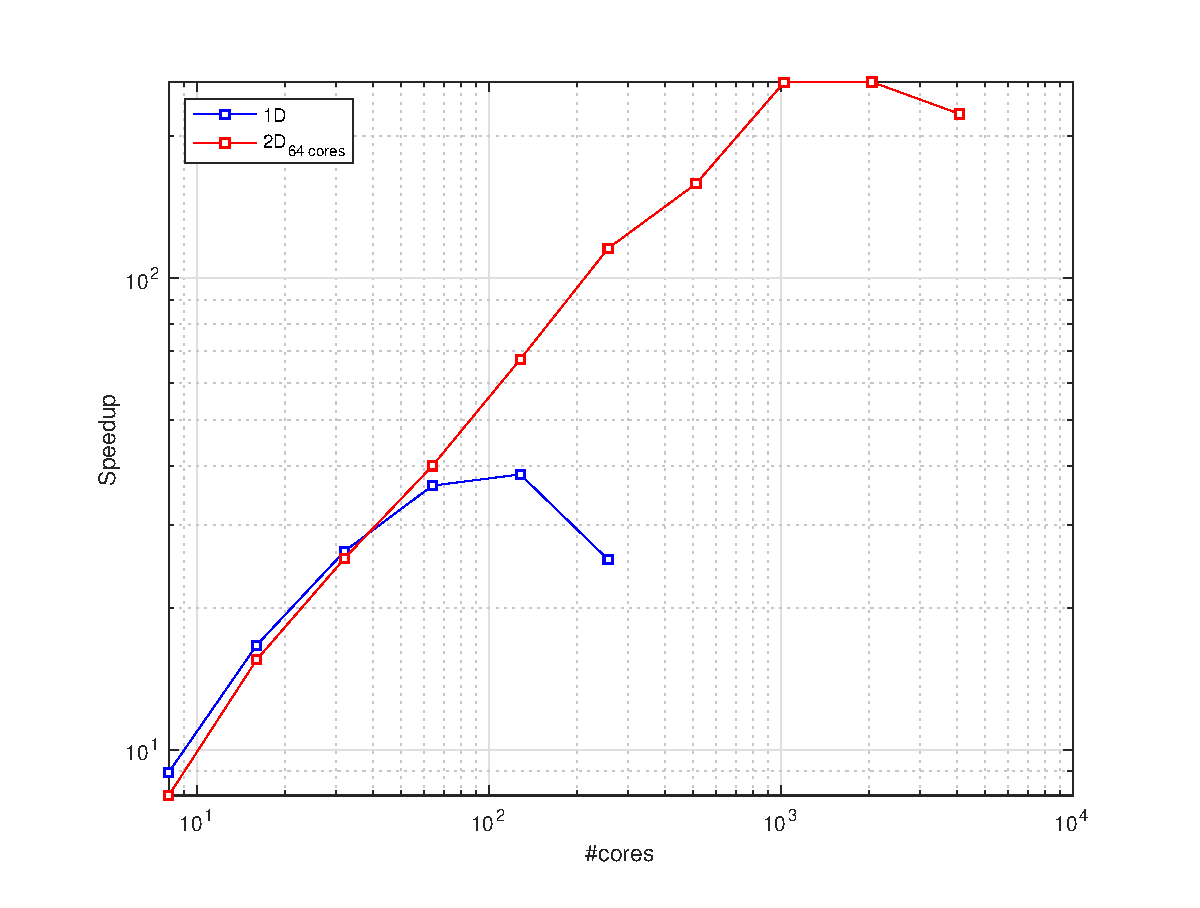
\includegraphics[scale=0.6]{grafici/5122}
\caption{Speedup performance factor of $512^3$ simulation}
\label{5122}
\end{center}
\end{figure}

As we can see from figure~\ref{5122}, the speedup factor of the 2D decomposed algorithm increase approximately linearly until $512$ cores. The raise in performance continue at lower factor until $2048$ cores are reached, where start descending.
The inverse behavior is shown in figure~\ref{5121}, where the simulation time is plotted against the number of cores.
\par
In figure~\ref{5121} is also reported the theoretical scaling limit. Comparing this line, in dashed green, with our results let us conclude that our scaling, although linear for the majority of the time, is sub-optimal. 
The same reasoning is valid also for the slab decomposed algorithm, although in a smaller region of cores number.
It is interesting to denote the advantageous behavior of such algorithm until $64$ cores, where performances are still slightly different in terms of speedup factor. 
\par
By looking at the values in table~\ref{512data} of page~\pageref{512data} and the depicted counter part, in figures~\ref{5121} and \ref{5122}, it is possible to denote that between $8$ and $16$ cores the loss are really small. This lead us to expect a perfect theoretical linear behavior from $1$ to $16$ cores. Keeping this in mind, we feel confident and seems reasonable to consider a speedup factor of $8$ for the $8$ cores simulation, possibly doing an error, however remaining below the unit. \\
\par
We refer to figure~\ref{5123} to have an idea of the efficiency of the algorithm. The figure shows that the efficiency remains above $80\%$ until $32$ cores are used. However, once passed such limit, the behavior is linear and smoother with respect to the ones shown in figure~\ref{644} of page~\pageref{644}. 
\par

\begin{figure}
\begin{center}
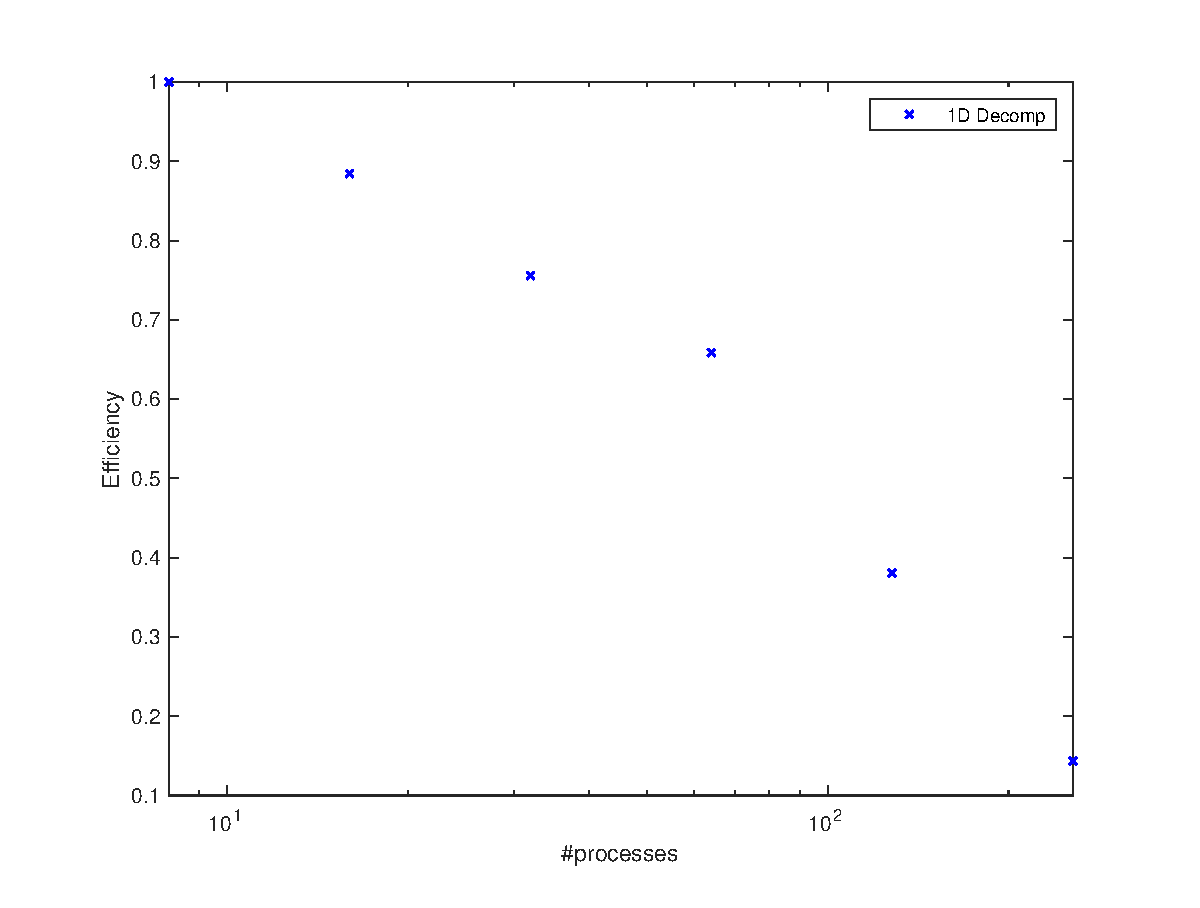
\includegraphics[scale=0.6]{grafici/5123}
\caption{Efficiency factor of $512^3$ simulation}
\label{5123}
\end{center}
\end{figure}

\begin{table}[h]
\caption{Data from $512^{3}$ simulation}
\begin{center}
\begin{tabular}{c c c c c}
\toprule
\textbf{\#cores} & \textbf{Time [s]} & \textbf{Speedup} & \textbf{Efficiency [\%]} & \textbf{Decomp}\\
\midrule
\multirow{2}{*}{8} & 1750 & 8.96 & 100 &1D\\
& 1960 & 1 & 100 & 2D\\
\hline
\multirow{2}{*}{16} & 941.5 & 16.65 & 93 & 1D\\
& 1011 & 15.51 & 97 & 2D\\
\hline
\multirow{2}{*}{32} & 595.3 & 26.35 & 74 & 1D\\
& 616.2 & 25.45 & 80 & 2D\\
\hline
\multirow{2}{*}{64} & 432.1 & 36.3 & 51 & 1D\\
& 392.3 & 39.97 & 62 & 2D\\
\hline
\multirow{2}{*}{128} & 409.2 & 38.34 & 27 & 1D\\
& 233.2 & 67.22 & 53 & 2D\\
\hline
\multirow{2}{*}{256} & 620.1 & 25.29 & 9 & 1D\\
& 135.7 & 115.5 & 45 & 2D\\
\hline
512 & 99 & 158.4 & 31 & 2D\\
1024 & 60.4 & 259.6 & 25  & 2D \\
2048 & 60.2 & 260.2 & 13  & 2D \\
4092 & 70.4 & 222.6 & 5 & 2D\\
\bottomrule
\end{tabular}
\end{center}
\label{512data}
\end{table}

Such efficiency behavior is due to the fact that we are dealing with a heavily threaded process without using the most efficient approach, OpenMP. \\
\par
To increase the efficiency of the code we must reduce the number of threads per processor. In this way OpenMPI can manage the resources better, thus the efficiency curve remains flatter with respect to the previous ones. The presented behavior could be seen in figure~\ref{512:eff} of page~\pageref{512:eff}.
\par
Although the efficiency variation is not so evident, the reduction of tasks per processor lead to a consistent gain in terms of timing execution, leading to remarkable gain in terms of performance, as can be seen in figure~\ref{512:perf} of page~\ref{512:perf} that shows the speedup factor variation depending on the thread number. In particular passing from 64 threads per processor to 8 threads per processor allows the code to run approximately 25 times faster, and there is still room for further improvements.
\par
To sum up, by looking at figure~\ref{512:perf} and figure~\ref{512:eff}, it is possible to generalize that decreasing the number of threads per processor moves the speedup curves upwards, leading to better performances, and flatten the efficiency curves.
\begin{figure}
\begin{center}
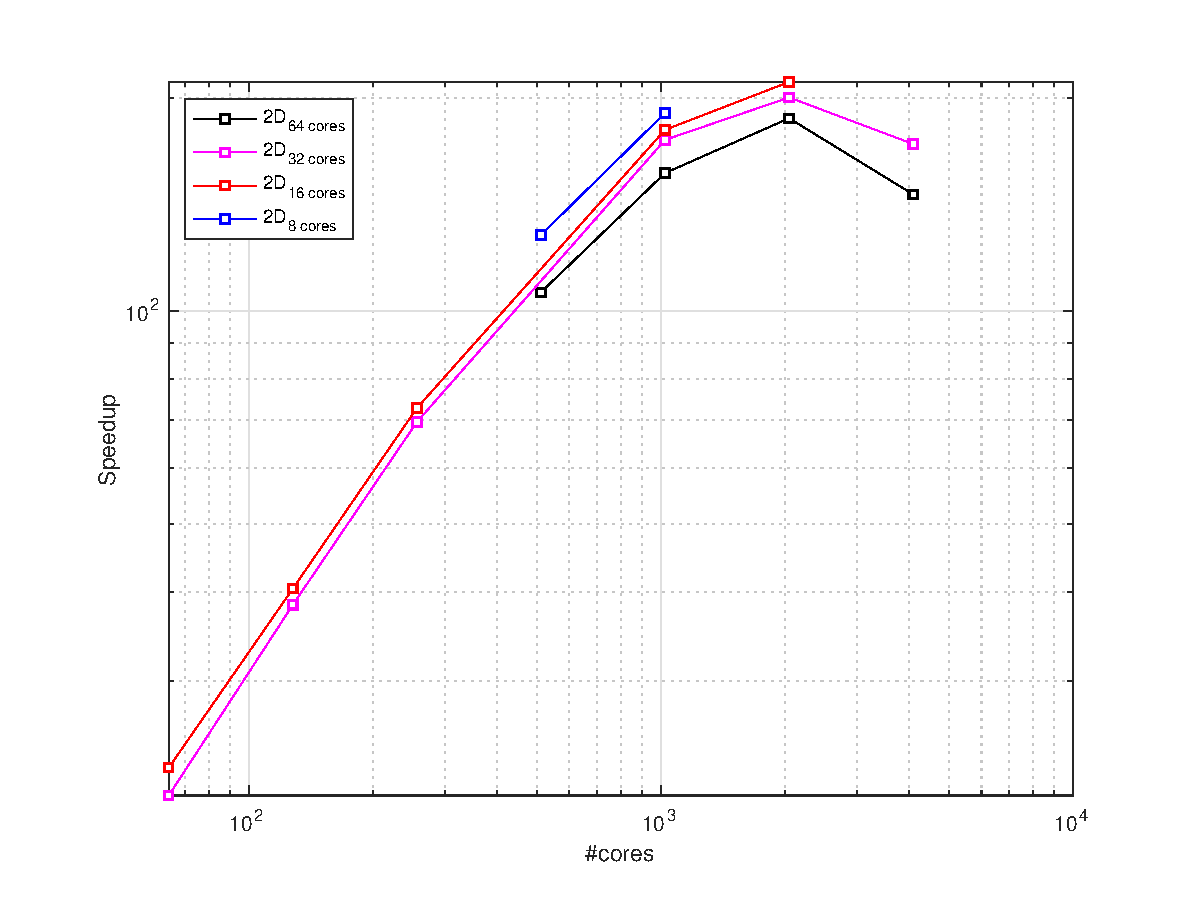
\includegraphics[scale=0.6]{grafici/5125}
\caption{Performance factor comparison for $512^3$ simulation}
\label{512:perf}
\end{center}
\end{figure}

\begin{figure}
\begin{center}
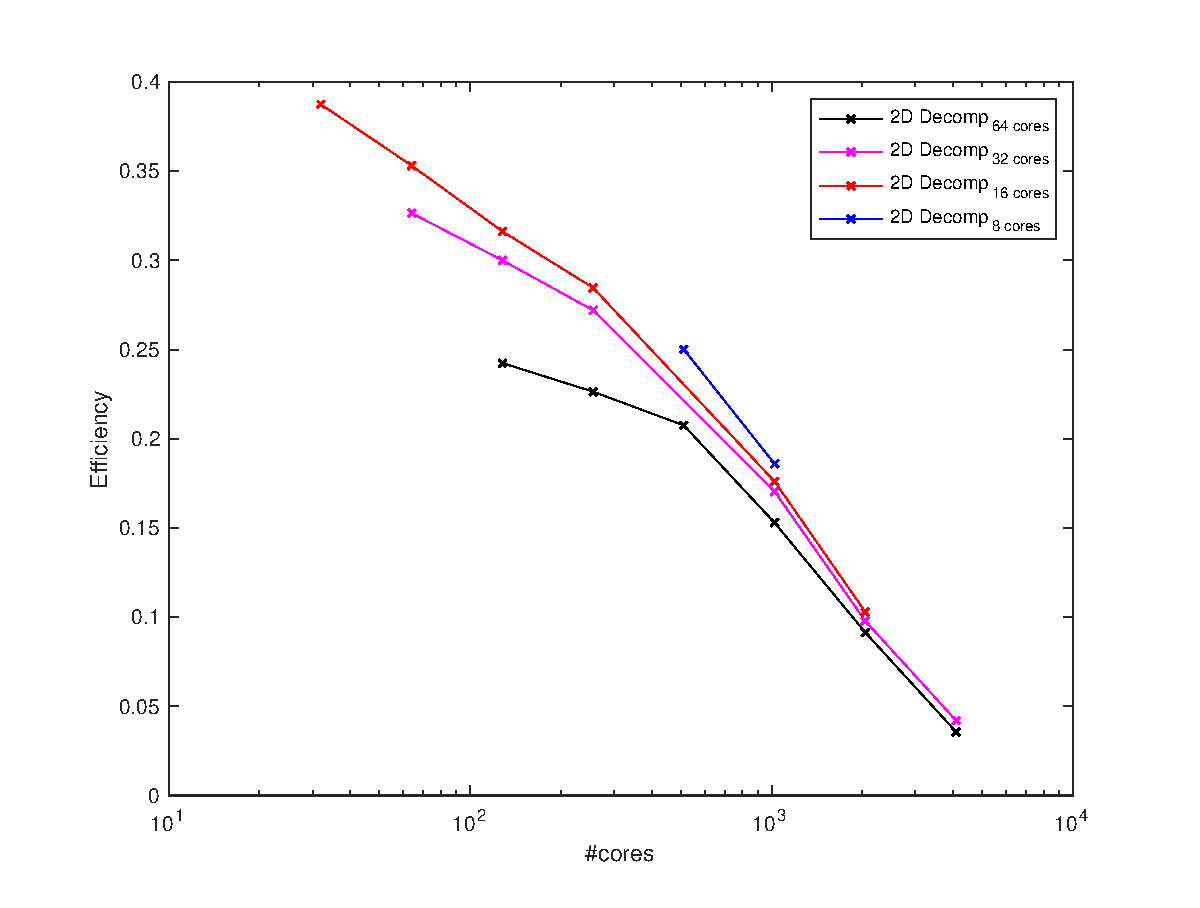
\includegraphics[scale=0.6]{grafici/5126}
\caption{Efficiency comparison for $512^3$ simulation}
\label{512:eff}
\end{center}
\end{figure}